In this lab we will be capturing and analyzing packets using Wireshark, TCPDump, and NetWitness Investigator

On Windows I am using Wireshark to capture packets, both time slots use the \verb|WiFi| connection.
\begin{figure}[H]
    \centering
    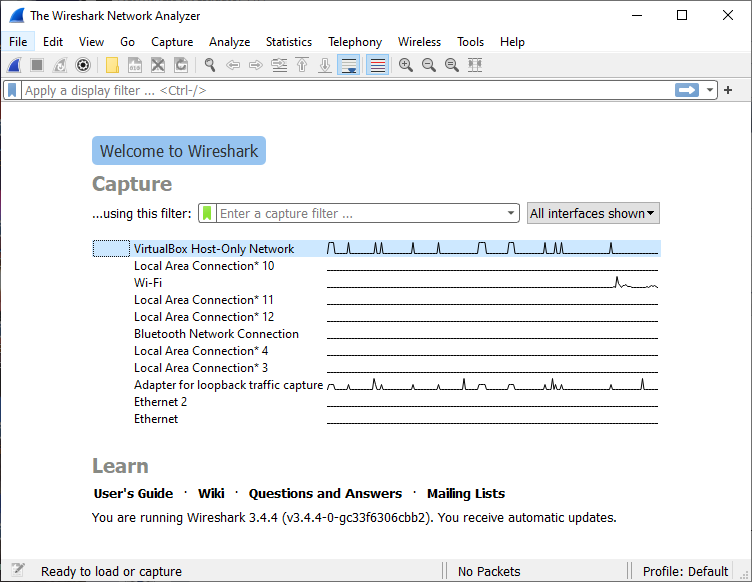
\includegraphics[width=\linewidth]{figures/wireshark_start.png}
    \caption{Start screen of Wireshark.}
\end{figure}

\begin{figure}[H]
    \centering
    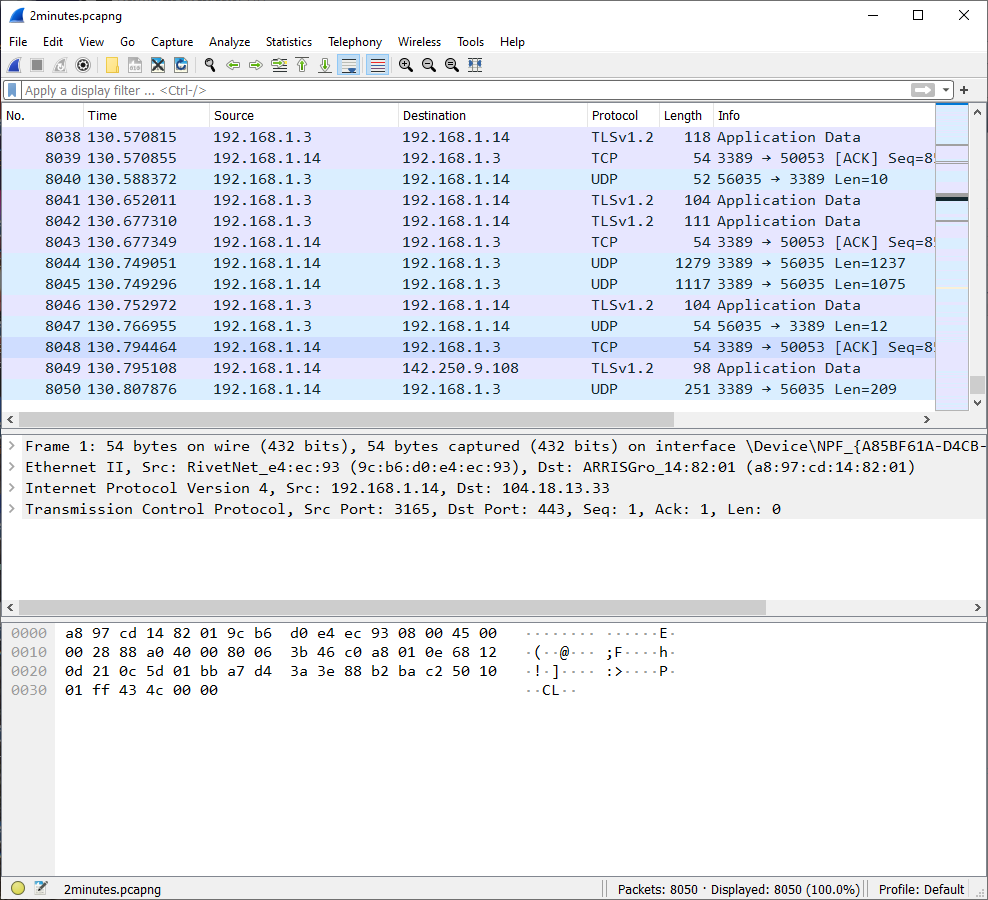
\includegraphics[width=\linewidth]{figures/2minutes_wireshark.png}
    \caption{Capture for 2 minutes.}
    \label{fig:2min}
\end{figure}

\begin{figure}[H]
    \centering
    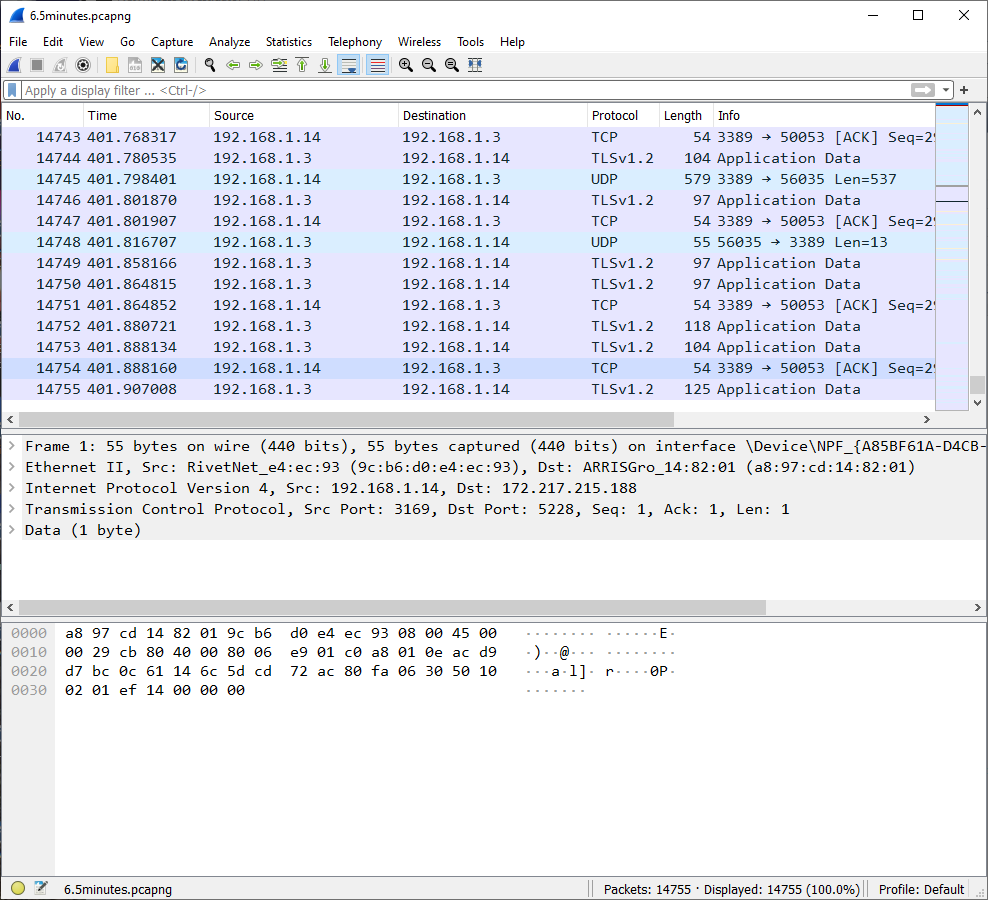
\includegraphics[width=\linewidth]{figures/6.5minutes_wireshark.png}
    \caption{Capture for 6.5 minutes}
    \label{fig:6.5}
\end{figure}

\begin{figure}[H]
    \centering
    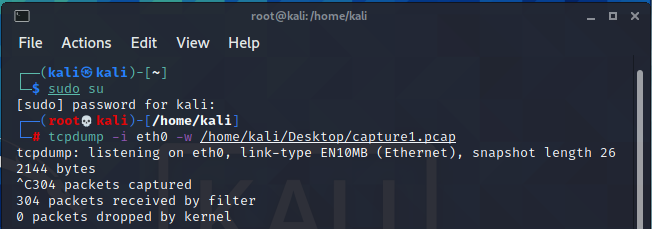
\includegraphics[]{figures/tcpdump.png}
    \caption{Fast TCPDump session, number of packets is because of a ping flood attack.}
    \label{fig:tcpdump}
\end{figure}

\begin{figure}[H]
    \centering
    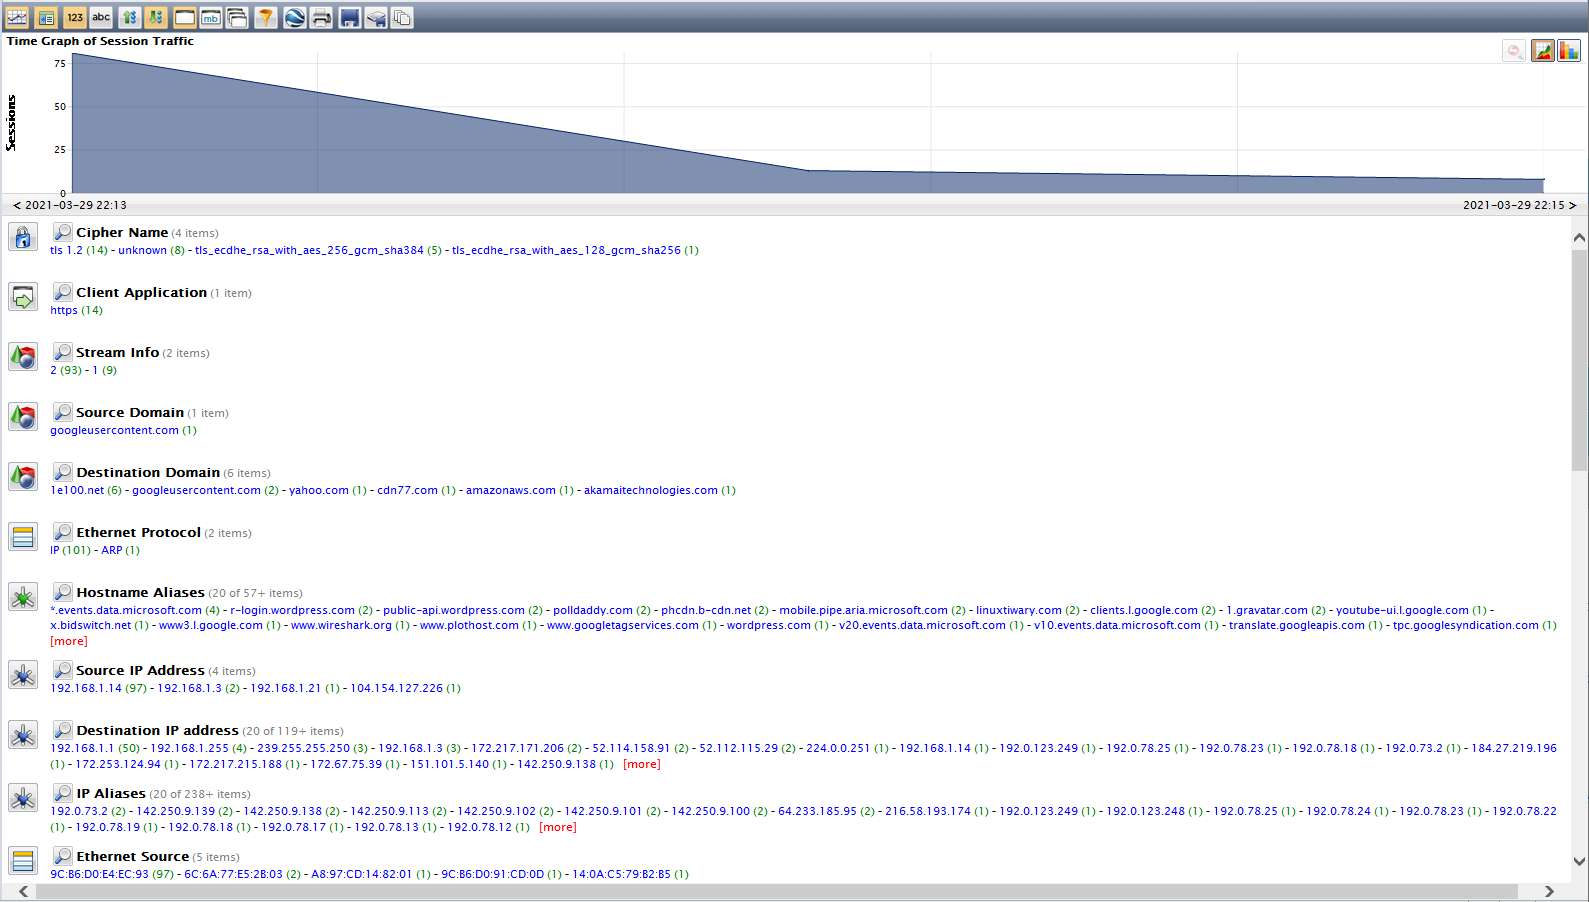
\includegraphics[width=\linewidth]{figures/2minutes_netwitness.png}
    \caption{Netwitness summary of 2 minute scan.}
    \label{fig:netwit2}
\end{figure}

\begin{figure}[H]
    \centering
    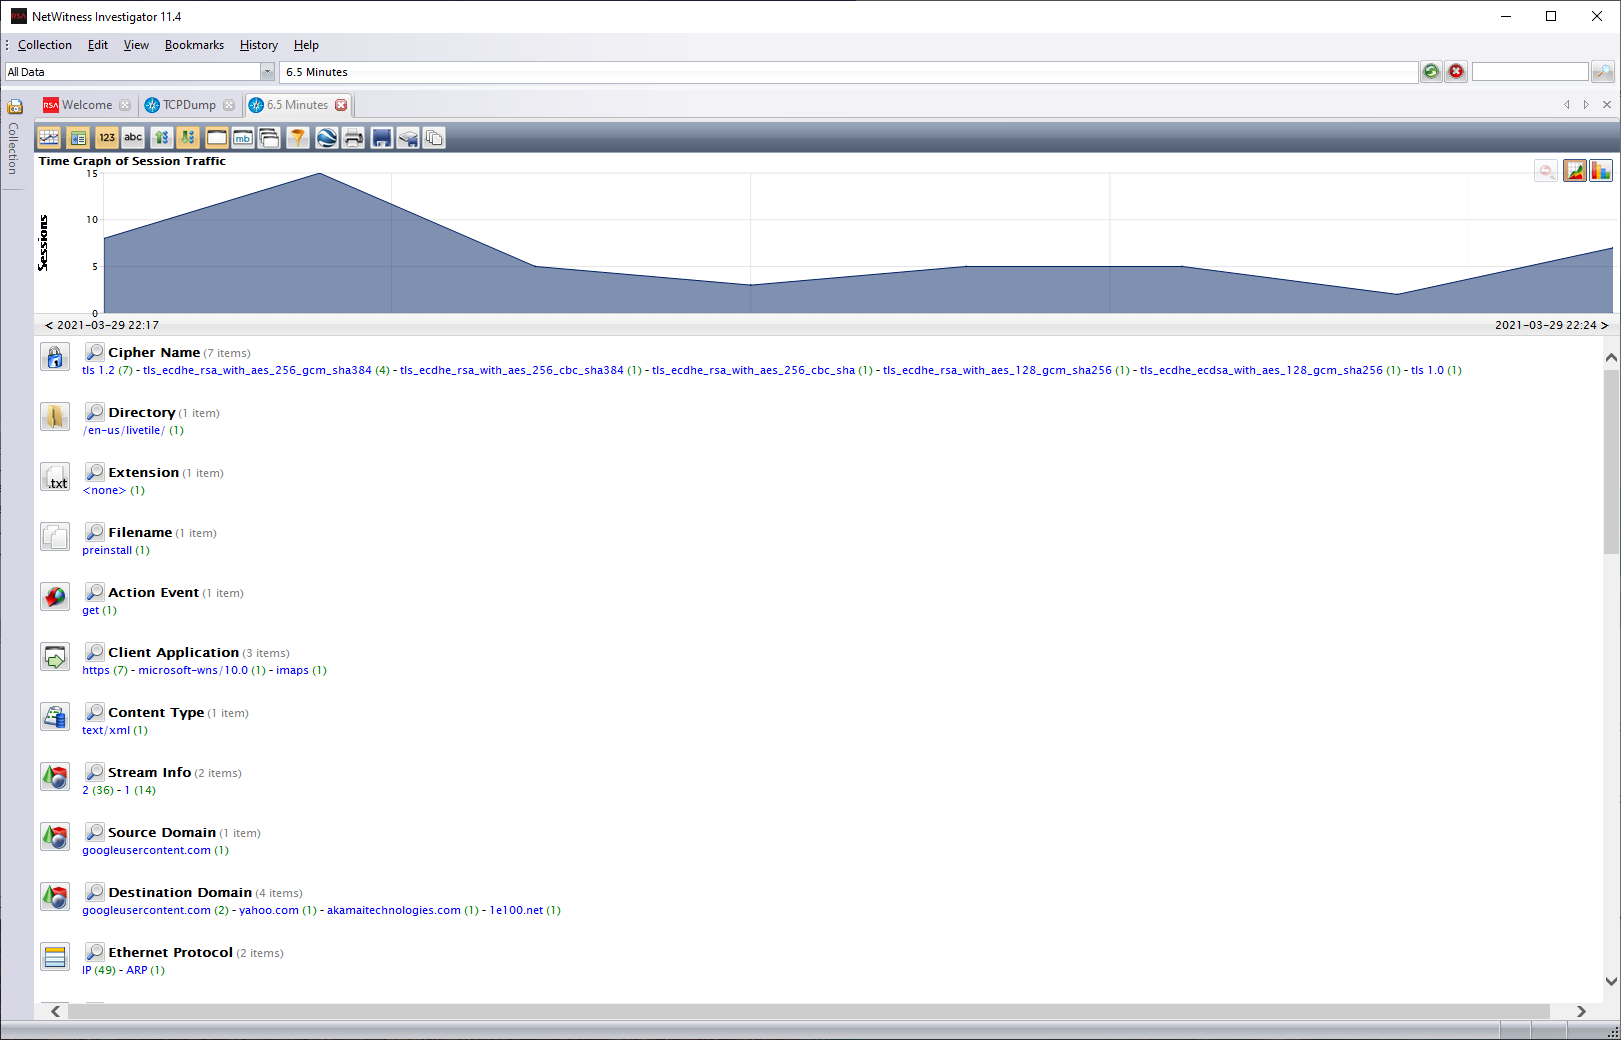
\includegraphics[width=\linewidth]{figures/6.5minutes_netwitness.png}
    \caption{Netwitness summary of 6.5 minute scan}
    \label{fig:netwit6}
\end{figure}

\begin{figure}[H]
    \centering
    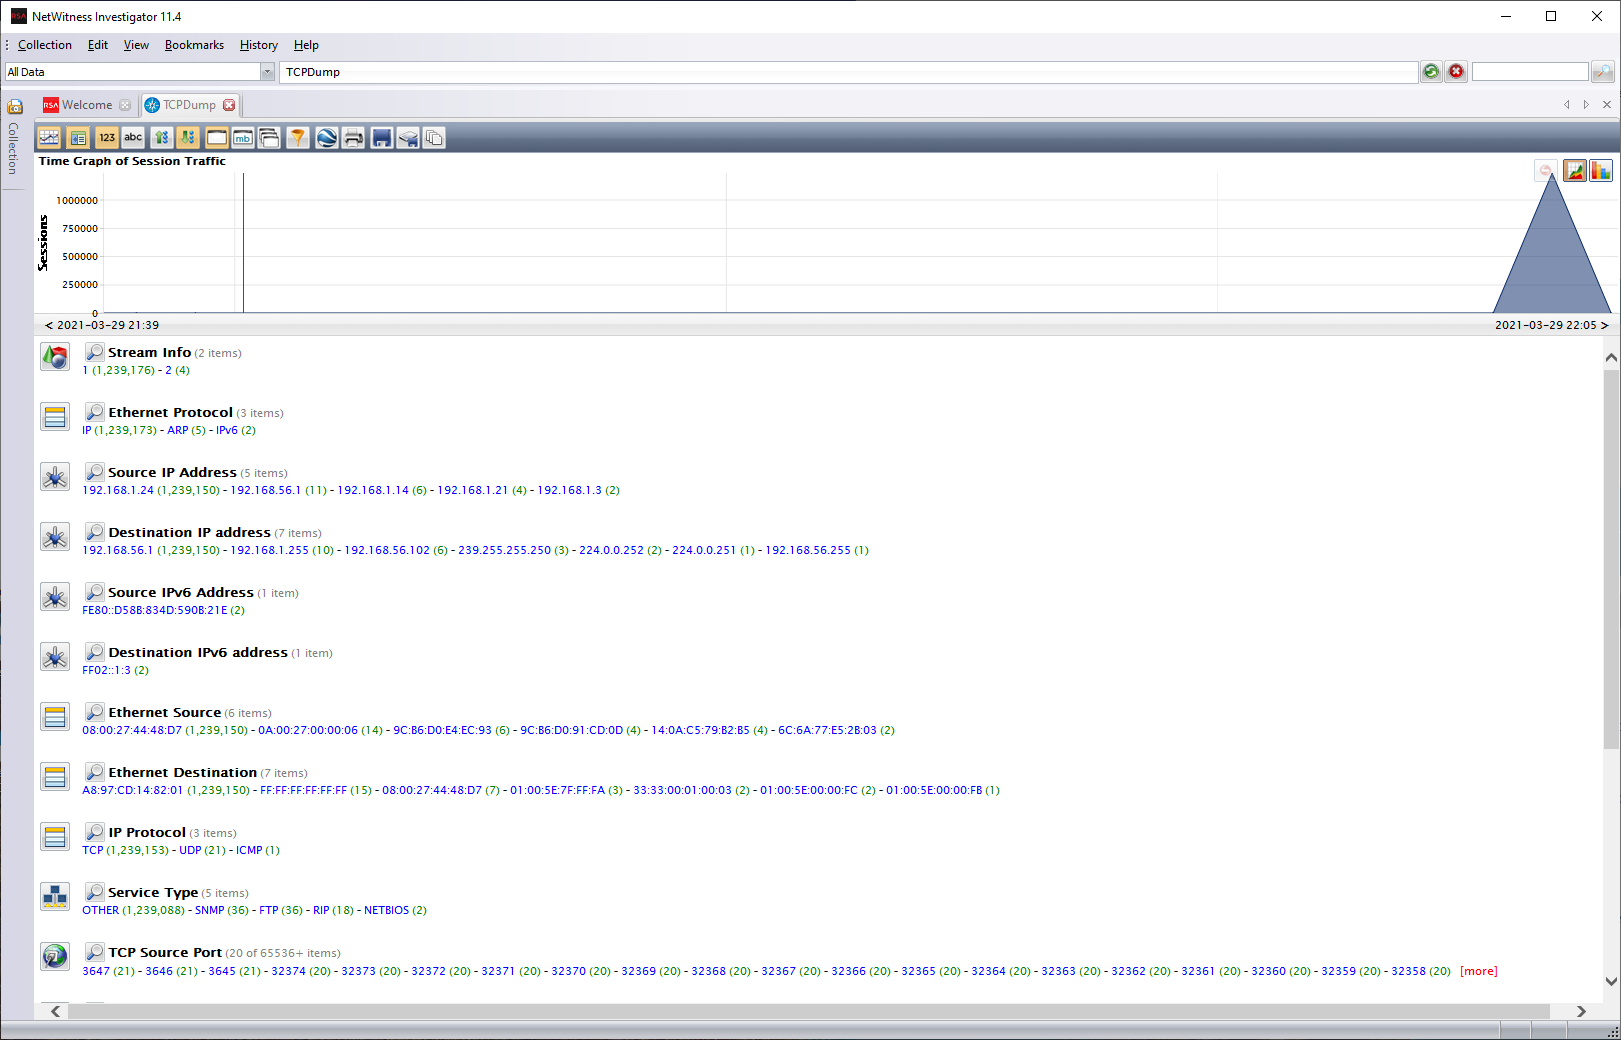
\includegraphics[width=\linewidth]{figures/tcpdump_netWitness.png}
    \caption{NetWitness summary of TCPDump.}
    \label{fig:netwitTCP}
\end{figure}
The graph at the top shows a large spike in network traffic.
Before the spike there are virtually no packets transferred, however during the spike there were almost 1.25 million packets transferred.

\begin{figure}[H]
    \centering
    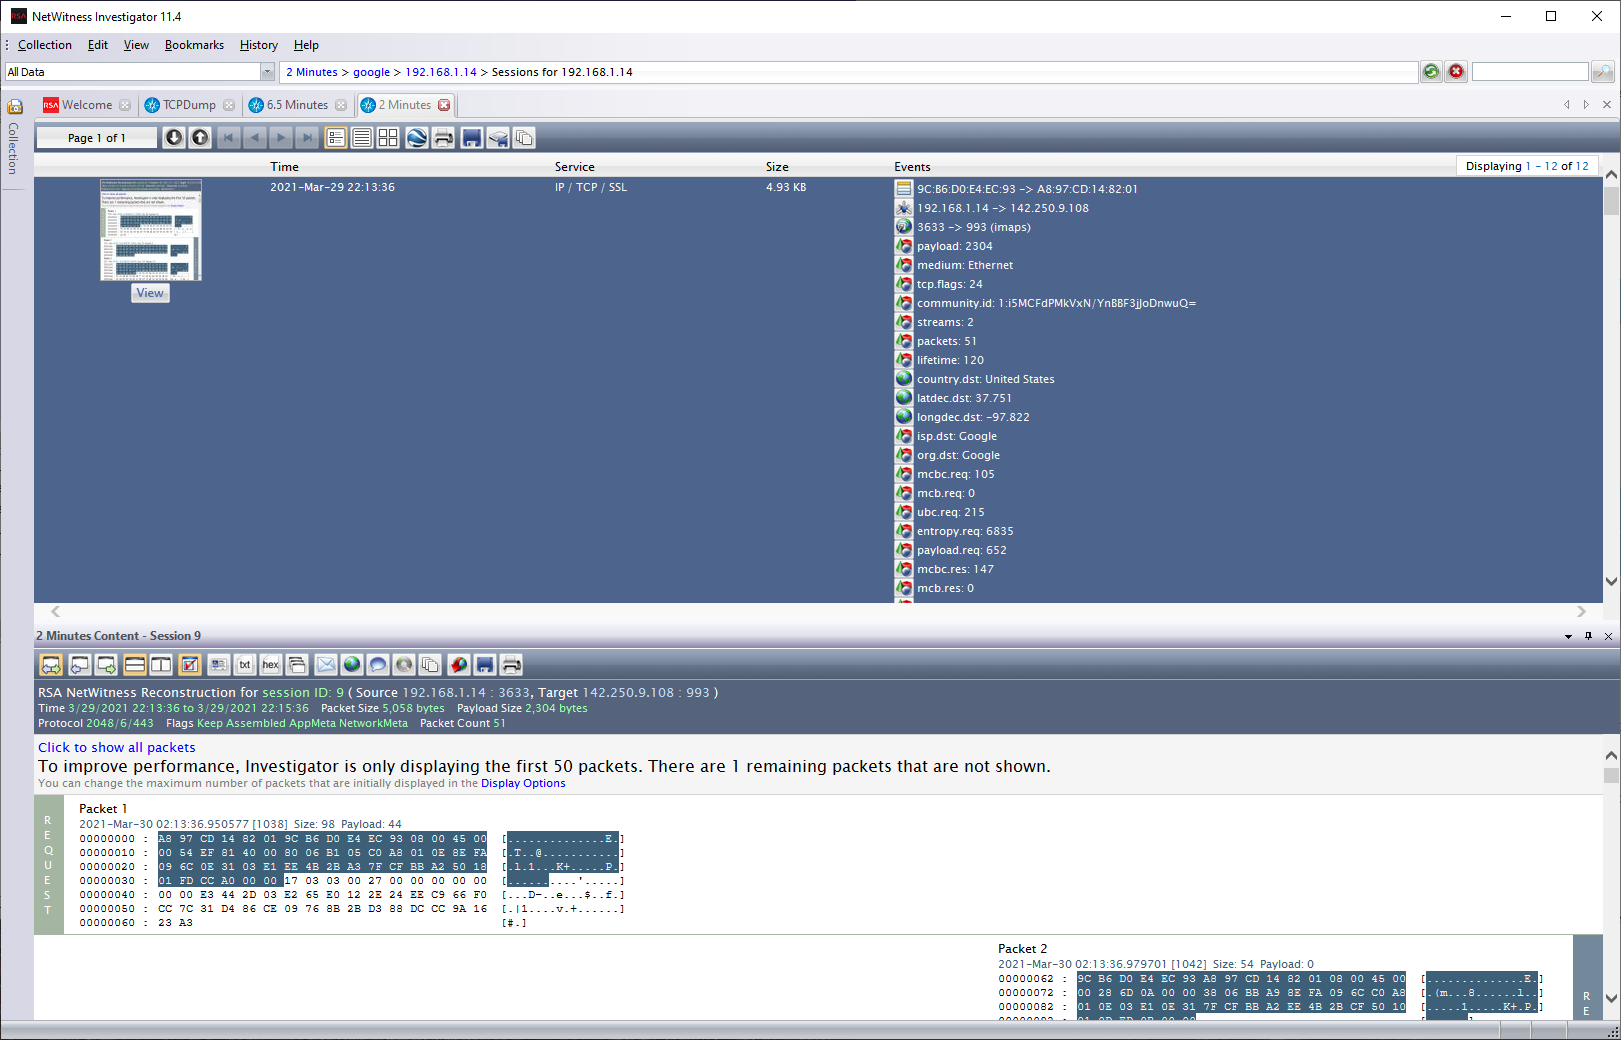
\includegraphics[width=\linewidth]{figures/2minutes_drilldown.png}
    \caption{NetWitness also allows us to drill down into categories and view individual packet data.}
    \label{netwitdrill}
\end{figure}

In this lab i learned how to use Wireshark on Windows machines and TCPDump on Kali Linux to capture network traffic.
Wireshark has filtering options available in the application but i chose to explore the NetWitness Investigator application.
NetWitness categories packets much more thn Wireshark does.
NetWitness gives consolidated lists of IP addresses that generate the most traffic.
As seen in figure \ref{fig:netwitTCP} the timeline is also an important tool to find times of large network traffic, or in this case, to view the packets in a ping flood attack.